\section{Инфологическая модель}\label{sec:infological-model}


\subsection{Информационные объекты}\label{subsec:information-objects}


\newcommand{\img}[2]{
    \begin{figure}[H]
        \center{\includegraphics[scale=0.9]{graphics/#1}}
        \caption{#2}
        \label{fig:#1}
    \end{figure}
}
\newcommand{\tab}{\hspace{1cm}}

\setlist[enumerate, 1]{align=left, leftmargin=0cm, labelindent=1cm, listparindent=1cm, labelwidth=*, itemindent=2cm}
\setlist[enumerate, 2]{align=left, leftmargin=1cm, labelindent=2cm, listparindent=1cm, labelwidth=*, itemindent=2cm}
\setlist[itemize, 1]{align=left, leftmargin=1cm, labelindent=2cm, listparindent=1cm, labelwidth=*, itemindent=2cm}


Выделим следующие информационные объекты:
\begin{enumerate}
    \item \textbf{Телефонный номер} -- это уникальный идентификационный номер в телекоммуникационной системе связи. Этот объект характеризуется следующими атрибутами:
    \begin{enumerate}
        \item Телефонный номер:
        \begin{itemize}
            \item является уникальным идентификационным номером в телекоммуникационной системе связи;
            \item получает оператор сотовой связи;
            \item хранится только значимая часть телефонного номера, то есть его код города/оператора вместе с абонентским номером;
            \item тип: целое число;
            \item интервал возможных значений: $[0; 9 999 999 999]$;
            \item используется как идентификационный номер в телекоммуникационной системе связи;
            \item менеджер и абонент не имеют никакого доступа, продавец-консультант имеет только доступ для чтения.
        \end{itemize}

        \item Абонентский счёт:
        \begin{itemize}
            \item является номером банковского счёта, на который зарегистрирован данный телефонный номер;
            \item выдаётся банком, с которым компания сотового оператора состоит в партнёрских отношениях;
            \item тип: натуральное число;
            \item интервал возможных значений: $[10 000 000 000 000 000 000; 99 999 999 999 999 999 999]$;
            \item используется как определитель абонента, использующего данный телефонный номер;
            \item менеджер и абонент не имеют никакого доступа, продавец-консультант имеет только доступ для чтения.
        \end{itemize}
    \end{enumerate}
    \img{phone-number-attributes}{Взаимосвязи атрибутов объекта <<Телефонный номер>>}


    \item \textbf{Тариф} -- это включаемые услуги и ставки оплаты за эти же услуги, предоставляемые компанией. Этот объект характеризуется следующими атрибутами:
    \begin{enumerate}
        \item Название:
        \begin{itemize}
            \item является читаемым и запоминающимся определителем тарифа, а также его уникальным идентификатором;
            \item разрабатывается менеджером (или группой менеджеров) компании сотового оператора;
            \item тип: текстовый;
            \item максимальный размер: 64 символа;
            \item используется как запоминающийся определитель тарифа;
            \item все пользователи имеют доступ на чтение, но менеджер также имеет доступ записи.
        \end{itemize}

        \item Абонентская плата:
        \begin{itemize}
            \item является размером ежемесячной платы за тариф;
            \item разрабатывается менеджером (или группой менеджеров) компании сотового оператора;
            \item тип: натуральное число;
            \item интервал возможных значений: $[150; 5000]$ (руб.); % TODO написать в анализе интервал значений для абонентской платы
            \item используется как описание размера ежемесячной платы за тариф;
            \item все пользователи имеют доступ на чтение, но менеджер также имеет доступ записи.
        \end{itemize}

        \item Интернет трафик:
        \begin{itemize}
            \item является размером предоставляемой компанией соответствующей услуги;
            \item разрабатывается менеджером (или группой менеджеров) компании сотового оператора;
            \item тип: числовой;
            \item интервал возможных значений: $\{-1\} \cup [0; 50]$ (ГБ), максимум 2 знака после запятой; % TODO написать в анализе, что максимум 50 гб возможно или безлимит
            \item значение интерпретируется следующим образом: $-1$ -- <<безлимит>>, $[0; 50]$ -- <<выделенный интернет трафик>>;
            \item используется как описание размера предоставляемой компанией соответствующей услуги;
            \item все пользователи имеют доступ на чтение, но менеджер также имеет доступ записи.
        \end{itemize}

        \item Количество минут:
        \begin{itemize}
            \item является размером предоставляемой компанией соответствующей услуги;
            \item разрабатывается менеджером (или группой менеджеров) компании сотового оператора;
            \item тип: целое число;
            \item интервал возможных значений: $\{-1\} \cup [0; 2 000]$ (мин.); % TODO написать в анализе, что максимум 2000 мин. возможно или безлимит
            \item значение интерпретируется следующим образом: $-1$ -- <<безлимит>>, $[0; 2 000]$ -- <<выделенное количество минут>>;
            \item используется как описание размера предоставляемой компанией соответствующей услуги;
            \item все пользователи имеют доступ на чтение, но менеджер также имеет доступ записи.
        \end{itemize}

        \item Количество SMS:
        \begin{itemize}
            \item является размером предоставляемой компанией соответствующей услуги;
            \item разрабатывается менеджером (или группой менеджеров) компании сотового оператора;
            \item тип: целое число;
            \item интервал возможных значений: $\{-1\} \cup [0; 2 000]$ (шт.); % TODO написать в анализе, что максимум 2000 шт. возможно или безлимит
            \item значение интерпретируется следующим образом: $-1$ -- <<безлимит>>, $[0; 2 000]$ -- <<выделенное количество SMS>>;
            \item используется как описание размера предоставляемой компанией соответствующей услуги;
            \item все пользователи имеют доступ на чтение, но менеджер также имеет доступ записи.
        \end{itemize}
    \end{enumerate}
    \img{tariff-attributes}{Взаимосвязи атрибутов объекта <<Тариф>>}


    \item \textbf{Клиент} -- это лицо, заинтересованное в получении услуг данной компании. Клиент характеризуется следующими атрибутами:
    \begin{enumerate}
        \item Серия и номер паспорта:
        \begin{itemize}
            \item является идентификационным номером документа клиента, подтверждающего его личность;
            \item берётся из паспорта клиента;
            \item тип: натуральное число;
            \item интервал возможных значений: $[100 000 101; 9 999 999 999]$;
            \item используется как идентификационный номер клиента в системе;
            \item менеджер не имеет никакого доступа, продавец-консультант имеет доступ для чтения и записи, абонент имеет только доступ для чтения.
        \end{itemize}

        \item ФИО:
        \begin{itemize}
            \item является именем, по которому обращаются к клиенту;
            \item берётся из паспорта клиента;
            \item тип: строковый;
            \item максимальный размер: 128 символов;
            \item используется как имя, по которому обращаются к клиенту;
            \item менеджер не имеет никакого доступа, продавец-консультант имеет доступ для чтения и записи, абонент имеет только доступ для чтения.
        \end{itemize}

        \item Дата рождения клиента:
        \begin{itemize}
            \item является датой календарного дня, в который был рождён клиент;
            \item берётся из паспорта клиента;
            \item тип: дата;
            \item интервал возможных значений: [120 лет назад, относительно сегодняшней даты; 18 лет назад, относительно сегодняшней даты];
            \item используется для определения возраста клиента;
            \item менеджер не имеет никакого доступа, продавец-консультант имеет доступ для чтения и записи, абонент имеет только доступ для чтения.
        \end{itemize}

        \item Место прописки:
        \begin{itemize}
            \item является названием места, по которому прописан клиент;
            \item берётся из паспорта клиента;
            \item тип: строковый;
            \item максимальный размер: 255 символов;
            \item используется как служебная информация о клиенте;
            \item менеджер не имеет никакого доступа, продавец-консультант имеет доступ для чтения и записи, абонент имеет только доступ для чтения.
        \end{itemize}
    \end{enumerate}
    \img{client-attributes}{Взаимосвязи атрибутов объекта <<Клиент>>}


    \item \textbf{Абонент} -- это пользователь услугами сотового оператора. Абонент характеризуется следующими атрибутами:
    \begin{enumerate}
        \item Абонентский счёт:
        \begin{itemize}
            \item является номером банковского счёта абонента;
            \item выдаётся абоненту с заключением договора;
            \item тип: натуральное число;
            \item интервал возможных значений -- $[10 000 000 000 000 000 000; 99 999 999 999 999 999 999]$;
            \item используется как номер банковского счёта абонента для оплаты за услуги;
            \item менеджер не имеет никакого доступа, продавец-консультант имеет доступ для чтения и записи, абонент имеет только доступ для чтения.
        \end{itemize}

        \item Баланс на абонентском счёте:
        \begin{itemize}
            \item является отображением денежной суммы, хранящейся на счёте абонента;
            \item изначально равен 0, затем изменяется зависимо от операций абонента;
            \item тип: числовой;
            \item интервал возможных значений: $[-999 999; 999 999]$ (руб.), максимум 2 знака после запятой; % нигде в анализе об этом не написано
            \item используется для определения задолженности у абонента;
            \item менеджер и не имеет никакого доступа, продавец-консультант и абонент имеют доступ для чтения.
        \end{itemize}

        \item Телефонный номер:
        \begin{itemize}
            \item является уникальным идентификационным номером абонента в телекоммуникационной системе связи;
            \item выдаётся абоненту с заключением договора;
            \item хранится только значимая часть телефонного номера, то есть его код города/оператора вместе с абонентским номером; 
            \item тип: натуральное число;
            \item интервал возможных значений: $[0; 9 999 999 999]$;
            \item используется как идентификационный номер абонента в телекоммуникационной системе связи;
            \item менеджер не имеет никакого доступа, продавец-консультант имеет доступ для чтения и записи, абонент имеет только доступ для чтения.
        \end{itemize}

        \item Подключённый тариф:
        \begin{itemize}
            \item является названием тарифа, зарегистрированного на данного абонента;
            \item при желании абонента подключается после заключения договора абонемента;
            \item тип: текстовый или <<пусто>>;
            \item максимальный размер: 64 символа; % нигде в анализе об этом не написано
            \item используется для определения зарегистрированного тарифа на данного абонента;
            \item менеджер не имеет никакого доступа, продавец-консультант имеет только доступ для чтения, абонент имеет доступ для чтения и записи.
        \end{itemize}

        \item Серия и номер паспорта:
        \begin{itemize}
            \item является идентификационным номером документа абонента, подтверждающего его личность;
            \item берётся из паспорта абонента;
            \item тип: натуральное число;
            \item интервал возможных значений: $[100000101; 9 999 999 999]$;
            \item используется как идентификационный номер абонента в системе;
            \item менеджер не имеет никакого доступа, продавец-консультант имеет доступ для чтения и записи, абонент имеет только доступ для чтения.
        \end{itemize}

        \item ФИО:
        \begin{itemize}
            \item является именем, по которому обращаются к абоненту;
            \item берётся из паспорта абонента;
            \item тип: строковый;
            \item максимальный размер: 128 символов; % нигде об этом не написано в анализе
            \item используется как имя, по которому обращаются к абоненту;
            \item менеджер не имеет никакого доступа, продавец-консультант имеет доступ для чтения и записи, абонент имеет только доступ для чтения.
        \end{itemize}

        \item Дата рождения абонента:
        \begin{itemize}
            \item является датой календарного дня, в который был рождён абонент;
            \item берётся из паспорта абонента;
            \item тип: дата;
            \item интервал возможных значений: [120 лет назад, относительно сегодняшней даты; 18 лет назад, относительно сегодняшней даты];
            \item используется для определения возраста абонента;
            \item менеджер не имеет никакого доступа, продавец-консультант имеет доступ для чтения и записи, абонент имеет только доступ для чтения.
        \end{itemize}

        \item Место прописки:
        \begin{itemize}
            \item является названием места, по которому прописан абонент;
            \item берётся из паспорта абонента;
            \item тип: строковый;
            \item максимальный размер: 255 символов;
            \item используется как служебная информация о абоненте;
            \item менеджер не имеет никакого доступа, продавец-консультант имеет доступ для чтения и записи, абонент имеет только доступ для чтения.
        \end{itemize}
    \end{enumerate}
    \img{subscriber-attributes}{Взаимосвязи атрибутов объекта <<Абонент>>}

    \item \textbf{Пользователь} -- это лицо, использующее базу данных в удовлетворении своих информационных потребностей. Пользователь характеризуется следующими атрибутами:
    \begin{enumerate}
        \item Логин:
        \begin{itemize}
            \item является уникальным идентификатором пользователя в системе;
            \item создается системой;
            \item тип: текстовый;
            \item максимальный размер: 32 символа;
            \item используется как идентификатор пользователя в системе;
            \item менеджер, продавец-консультант и абонент не имеют никакого доступа.
        \end{itemize}

        \item Пароль:
        \begin{itemize}
            \item является секретным ключом пользователя в системе;
            \item создается системой или пользователем;
            \item тип: текстовый;
            \item максимальный размер: 32 символа;
            \item используется для проверки личности пользователя в системе;
            \item менеджер, продавец-консультант и абонент не имеют никакого доступа.
        \end{itemize}

        \item Тип пользователя:
        \begin{itemize}
            \item является определителем прав пользователя в системе;
            \item выдается системой;
            \item тип: текстовый;
            \item максимальный размер: 32 символа;
            \item используется для определения прав пользователя в системе;
            \item менеджер, продавец-консультант и абонент не имеют никакого доступа.
        \end{itemize}
    \end{enumerate}
    \img{user-attributes}{Взаимосвязи атрибутов объекта <<Пользователь>>}
\end{enumerate}


\subsection{Задачи пользователей}\label{user-problems}


\setlist[enumerate, 1]{align=left, leftmargin=0cm, labelindent=1cm, listparindent=1cm, labelwidth=*, itemindent=2cm}


\begin{enumerate}
    \item Задачи, которые решает \textbf{любой пользователь}:
        \img{any-user-task-1}{Просмотр актуальных тарифов}

    \item Задачи, которые решает \textbf{менеджер}:
        \img{manager-task-1}{Добавление нового тарифа в систему}
        \img{manager-task-2}{Изменение тарифа в системе}

    \item Задачи, которые решает \textbf{продавец-консультант}:
        \img{shop-assistant-task-1}{Регистрация нового клиента в системе}
        \img{shop-assistant-task-2}{Обновление данных о клиенте в системе}
        \img{shop-assistant-task-3}{Добавление абонента в систему}
        \img{shop-assistant-task-4}{Удаление абонента из системы}
        \img{shop-assistant-task-5}{Просмотр свободных телефонных номеров}
        \img{shop-assistant-task-6}{Просмотр информации об абонентах}

    \item Задачи, которые решает \textbf{абонент}:
        \img{subscriber-task-1}{Просмотр информации о своём абонентском аккаунте}
        \img{subscriber-task-2}{Подключение тарифа на свой абонентский счёт}
\end{enumerate}


\subsection{Нормализация}\label{normalization}

\setlist[enumerate, 1]{align=left, leftmargin=0cm, labelindent=1cm, listparindent=1cm, labelwidth=*, itemindent=2cm}
\setlist[itemize, 1]{align=left, leftmargin=1cm, labelindent=2cm, listparindent=1cm, labelwidth=*, itemindent=2cm}


% ТЕЛЕФОННЫЙ НОМЕР
Информационному объекту <<\textbf{Телефонный номер}>> ставим в соответствие таблицу \ref{table:phone-number-table}:
\begin{table}[H]
    \caption{Таблица объекта <<Телефонный номер>>}
    \label{table:phone-number-table}
    \renewcommand{\arraystretch}{1.5}
    \renewcommand{\tabularxcolumn}[1]{m{#1}}
    \begin{tabularx}{\textwidth}{|C|C|}
        \hline
        Телефонный номер & Абонентский счёт \\ \hline
    \end{tabularx}
\end{table}

\begin{enumerate}
    \item Приведение к первой нормальной форме:
    \begin{itemize}
        \item Все значения атрибутов уже атомарны.
        \item Проанализировав схему взаимосвязей атрибутов объекта <<Телефонный номер>> (рис. \ref{fig:phone-number-attributes}), выделяем первичный ключ. Возможными могут быть: <<Телефонный номер>> (атрибут <<Абонентский номер>> не включаем, так как он может быть пустым). Выбираем в качестве первичного ключа <<Телефонный номер>>.
    \end{itemize}
    \tab\tab Приведение к первой нормальной форме завершено.

    \item Приведение ко второй нормальной форме:
    \begin{itemize}
        \item Атрибут <<Абонентский номер>> зависит только от первичного ключа <<Телефонный номер>>.
    \end{itemize}
    \tab\tab Приведение ко второй нормальной форме завершено.

    \item Приведение к третьей нормальной форме:
    \begin{itemize}
        \item Транзитивной зависимости нет.
    \end{itemize}
    \tab\tab Приведение к третьей нормальной форме завершено.
\end{enumerate}


% ТАРИФ
Информационному объекту <<\textbf{Тариф}>> ставим в соответствие таблицу \ref{table:tariff-table}:
\begin{table}[H]
    \caption{Таблица объекта <<Тариф>>}
    \label{table:tariff-table}
    \renewcommand{\arraystretch}{1.5}
    \renewcommand{\tabularxcolumn}[1]{m{#1}}
    \begin{tabularx}{\textwidth}{|C|C|C|C|C|}
        \hline
        Название & Абонентская плата & Интернет трафик & Количество минут & Количество SMS \\ \hline
    \end{tabularx}
\end{table}

\begin{enumerate}
    \item Приведение к первой нормальной форме:
    \begin{itemize}
        \item Все значения атрибутов уже атомарны.
        \item Проанализировав схему взаимосвязей атрибутов объекта <<Тариф>> (рис. \ref{fig:tariff-attributes}), выделяем первичный ключ. Возможными могут быть: <<Название>>. Выбираем в качестве первичного ключа <<Название>>.
    \end{itemize}
    \tab\tab Приведение к первой нормальной форме завершено.

    \item Приведение ко второй нормальной форме:
    \begin{itemize}
        \item Атрибут <<Абонентская плата>>, <<Интернет трафик>>, <<Количество минут>>, <<Количество SMS>> зависят только от первичного ключа <<Название>>.
    \end{itemize}
    \tab\tab Приведение ко второй нормальной форме завершено.

    \item Приведение к третьей нормальной форме:
    \begin{itemize}
        \item Транзитивной зависимости нет.
    \end{itemize}
    \tab\tab Приведение к третьей нормальной форме завершено.
\end{enumerate}


% КЛИЕНТ
Информационному объекту <<\textbf{Клиент}>> ставим в соответствие таблицу \ref{table:client-table}:
\begin{table}[H]
    \caption{Таблица объекта <<Клиент>>}
    \label{table:client-table}
    \renewcommand{\arraystretch}{1.5}
    \renewcommand{\tabularxcolumn}[1]{m{#1}}
    \begin{tabularx}{\textwidth}{|C|C|C|C|}
        \hline
        Серия и номер паспорта & ФИО & Дата рождения клиента & Место прописки \\ \hline
    \end{tabularx}
\end{table}

\begin{enumerate}
    \item Приведение к первой нормальной форме:
    \begin{itemize}
        \item В нашей задаче не нужно разделять номер и серию паспорта, то есть будем считать, что значение атрибута <<Серия и номер паспорта>> уже атомарно.
        \item В нашей задаче не нужно разделять имя, фамилию и отчество, то есть будем считать, что значение атрибута <<ФИО>> уже атомарно.
        \item Проанализировав схему взаимосвязей атрибутов объекта <<Клиент>> (рис. \ref{fig:client-attributes}), выделяем первичный ключ. Возможными могут быть: <<Серия и номер паспорта>>. Выбираем в качестве первичного ключа <<Серия и номер паспорт>>.
    \end{itemize}
    \tab\tab Приведение к первой нормальной форме завершено.

    \item Приведение ко второй нормальной форме:
    \begin{itemize}
        \item Атрибут <<ФИО>>, <<Дата рождения клиента>> и <<Место прописки>> зависят только от первичного ключа <<Серия и номер паспорта>>
    \end{itemize}
    \tab\tab Приведение ко второй нормальной форме завершено.

    \item Приведение к третьей нормальной форме:
    \begin{itemize}
        \item Атрибут <<Место прописки>> не зависит напрямую от первичного ключа <<Серия и номер паспорта>>
        \item Производим декомпозицию (рис. \ref{fig:client-decomposition}).
        \img{client-decomposition}{Декомпозиция объекта <<Клиент>>}
    \end{itemize}
    \tab\tab Приведение к третьей нормальной форме завершено.
\end{enumerate}


% АБОНЕНТ
Информационному объекту <<\textbf{Абонент}>> ставим в соответствие таблицу \ref{table:subscriber-table}:
\begin{table}[H]
    \caption{Таблица объекта <<Абонент>>}
    \label{table:subscriber-table}
    \renewcommand{\arraystretch}{1.5}
    \renewcommand{\tabularxcolumn}[1]{m{#1}}
    \begin{tabularx}{\textwidth}{|C|C|C|C|C|C|C|C|}
        \hline
        Або-нент-ский счёт & Баланс на абонентском счёте & Теле-фон-ный номер & Под-клю-чён-ный тариф & Серия и номер паспорта & ФИО & Дата рождения абонента & Место прописки \\ \hline
    \end{tabularx}
\end{table}

\begin{enumerate}
    \item Приведение к первой нормальной форме:
    \begin{itemize}
        \item Проанализировав схему взаимосвязей атрибутов объекта <<Абонент>> (рис. \ref{fig:subscriber-attributes}), выделяем первичный ключ. Возможными могут быть: <<Абонентский счёт>> и <<Телефонный номер>>. Выбираем в качестве первичного ключа <<Абонентский счёт>>.
    \end{itemize}
    \tab\tab Приведение к первой нормальной форме завершено.

    \item Приведение ко второй нормальной форме:
    \begin{itemize}
        \item Атрибуты <<Баланс на абонентском счёте>>, <<Телефонный номер>>, <<Подключённый тариф>>, <<Серия и номер паспорта>>, <<ФИО>>, <<Дата рождения абонента>> и <<Место прописки>> зависят только от первичного ключа <<Абонентский счёт>>.
    \end{itemize}
    \tab\tab Приведение ко второй нормальной форме завершено.

    \item Приведение к третьей нормальной форме:
    \begin{itemize}
        \item Атрибуты <<ФИО>>, <<Дата рождения абонента>> и <<Место прописки>> не зависят напрямую от первичного ключа <<Абонентский счёт>> (в точности является объектом <<Клиент>>).
        \item Проанализировав предметную область, приходим к тому, что сотовый оператор хранит телефонные номера в системе независимо от наличия абонента, поэтому объект <<Абонент>> зависим от объекта <<Телефонный номер>>.
        \item Также приходим к тому, что сотовый оператор хранит тарифы в системе независимо от наличия абонента, поэтому объект <<Абонент>> зависим от объекта <<Тариф>>.
        \item Находим отношения объекта <<Абонент>> (рис. \ref{fig:subscriber-relations}).
        \img{subscriber-relations}{Отношения объекта <<Абонент>>}
    \end{itemize}
    \tab\tab Приведение к третьей нормальной форме завершено.
\end{enumerate}


% ПОЛЬЗОВАТЕЛЬ
Информационному объекту <<\textbf{Пользователь}>> ставим в соответствие таблицу \ref{table:user-table}:
\begin{table}[H]
    \caption{Таблица объекта <<Пользователь>>}
    \label{table:user-table}
    \renewcommand{\arraystretch}{1.5}
    \renewcommand{\tabularxcolumn}[1]{m{#1}}
    \begin{tabularx}{\textwidth}{|C|C|C|}
        \hline
        Логин & Пароль & Тип пользователя \\ \hline
    \end{tabularx}
\end{table}

\begin{enumerate}
    \item Приведение к первой нормальной форме:
    \begin{itemize}
        \item Проанализировав схему взаимосвязей атрибутов объекта <<Пользователь>> (рис. \ref{fig:user-attributes}), выделяем первичный ключ. Возможными могут быть: <<Логин>>. Выбираем в качестве первичного ключа <<Логин>>.
    \end{itemize}
    \tab\tab Приведение к первой нормальной форме завершено.

    \item Приведение ко второй нормальной форме:
    \begin{itemize}
        \item Атрибуты <<Пароль>>, <<Тип пользователя>> зависят только от первичного ключа <<Логин>>.
    \end{itemize}
    \tab\tab Приведение ко второй нормальной форме завершено.

    \item Приведение к третьей нормальной форме:
    \begin{itemize}
        \item Атрибут <<Тип пользователя>> не зависит напрямую от первичного ключа <<Логин>>.
        \item Производим декомпозицию объекта <<Пользователь>> (рис. \ref{fig:user-decomposition}).
        \img{user-decomposition}{Декомпозиция объекта <<Пользователь>>}
    \end{itemize}
    \tab\tab Приведение к третьей нормальной форме завершено.
\end{enumerate}


В итоге получаем следующую модель:
\begin{figure}[H]
    \center{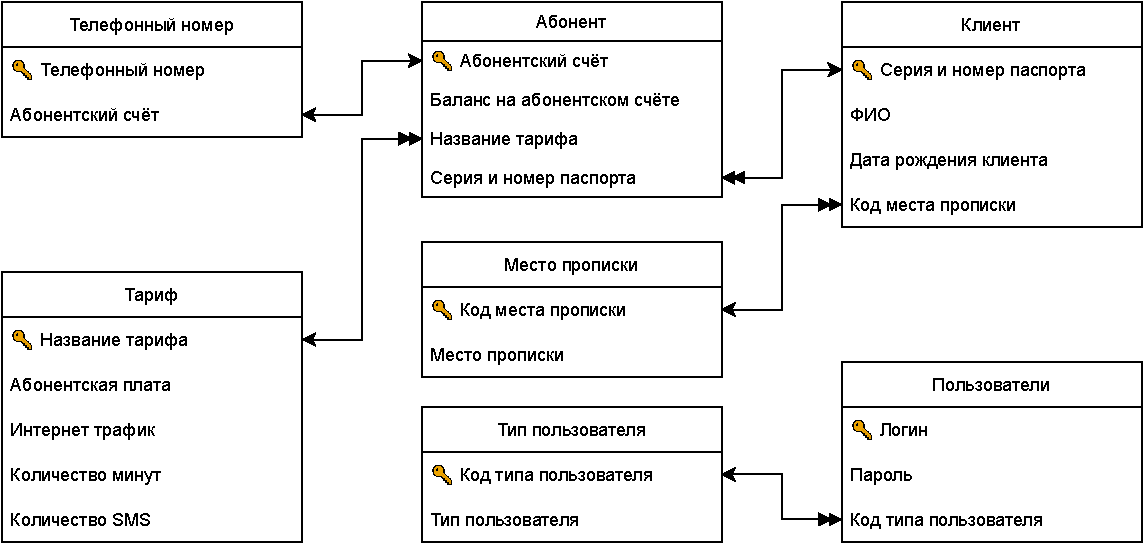
\includegraphics[scale=0.8]{graphics/model}}
    \caption{Модель}
    \label{fig:model}
\end{figure}